\section{Experiment Methodology}
\label{sec:methodology}

\subsection{Overview}

The experiment methodology follows Sudre et al.~\cite{Sudre2012} using the {\bf 
\tvt test}. We train a series of machine learning ridge regression models using 
the EEG data to generate the individual values for the given indices of {\bf 
word vectors} matching our word set as the models' predictions.

\subsection{Word Vectors}

We use the {\bf Skip-Gram} word vector set from Mikolov et 
al.~\cite{Mikolov2013}. These word vectors are generated by a neural network 
with a single hidden layer containing 300 neurons. The neural network is 
trained to perform a word collocation task: the network receives a single word 
as input and predicts the probable collocated words for that input word. Pairs 
of words are generated from the Google News text corpus using a sliding window 
over the text corpus. After training, the weights of the model can approximate 
the probability of collocated words. For each word in the vocabulary, the 
corresponding weights are extracted from the weight matrix which connects the 
input layer with the hidden layer. This extraction is done by multiplying the 
weight matrix with a one-hot input vector representing the target word. The 
resulting 300-dimensional word vectors are used as training data in our 
experiment.

Skip-Gram word vectors are a reasonable proxy for word semantics, and have 
interesting linguistic properties. For example, the difference between the 
vectors for ``man'' and ``woman'' is similar to the distance between the 
vectors for ``king'' and ``queen'', and the distance between ``walked'' and 
``walking'' is similar to the distance between ``swam'' and ``swimming''.

\begin{figure}[t]
  \centerline{
    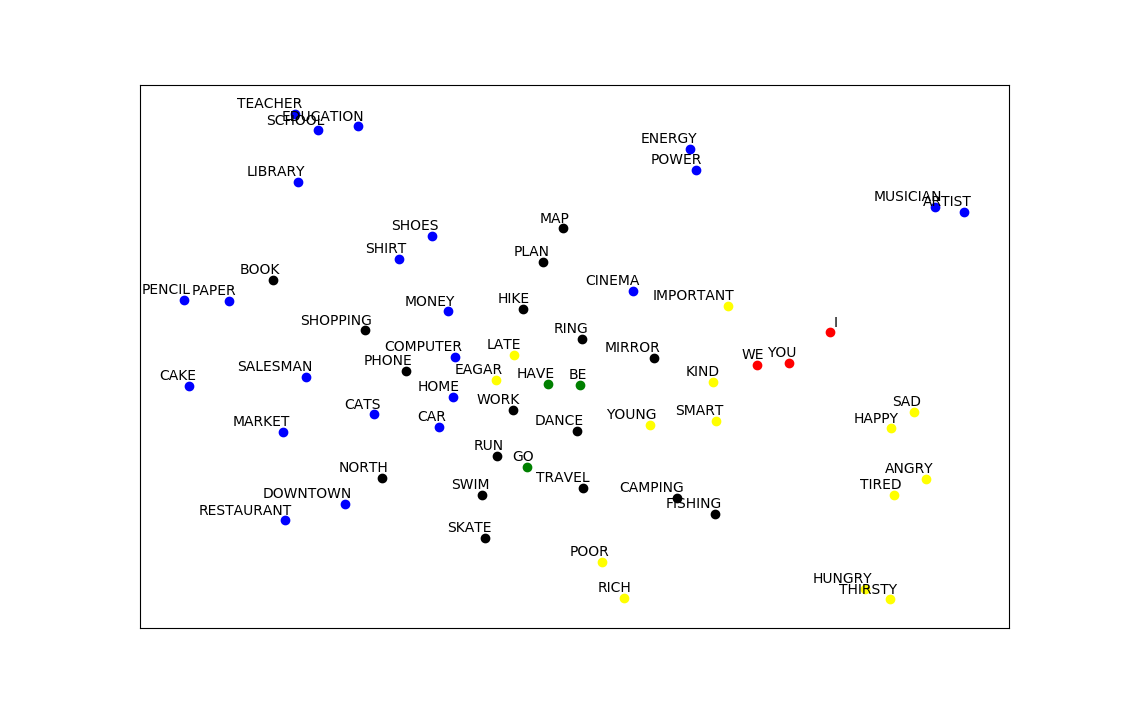
\includegraphics[width=\linewidth]{figures/tsne}
  }
  \caption[Visualization of Utilized Word Vectors]{
    A visualization of the word vectors utilized in this thesis, generated by a 
    t-Distributed Stochastic Neighbor Embedding~\cite{maaten2008visualizing}.  
    This technique reduces the input into two dimensions, allowing us to 
    visualize and approximate their relationships in high dimensional space.  
    Similar word semantics are seen clustered closer together. Blue represents 
    abstract and concrete nouns, yellow represents adjectives, red represents 
    pronouns, green represents verbs, and black represents words which act as 
    multiple parts of speech.
  }
  \label{fig:tsne}
\end{figure}

More rigorously, Hollis et al. showed that Skip-Gram could predict human 
judgments for semantic tasks (e.g. sentiment 
ratings)~\cite{hollis2017extrapolating}.  Hill et al.  additionally concluded 
that Skip-Gram performs well on their SlimLex-999 evaluation, a high quality 
word similarity benchmark for computational models of word 
meaning~\cite{hill2016simlex}. Further, Murphy et al. showed that computational 
models can perform similarly to human benchmarks in the specific context of 
neurolinguistic decoding tasks~\cite{Murphy2012}, and subsequent work showed 
specifically that Skip-Gram could be used to identify the semantics of many 
word types in fMRI and EEG~\cite{xu2016brainbench}. The semantic properties of 
these word vectors make them a useful tool for performing semantic analysis on 
brain data. A simplified representation of the word vectors used in this 
thesis, generated using the t-SNE dimensionality reduction 
technique~\cite{maaten2008visualizing}, is shown in Figure~\ref{fig:tsne}.

\subsection{Prediction Model}

After the data preprocessing steps mentioned in Section 
\ref{sec:preprocessing}, every participant-symbol pair is represented by a 
tensor $D \in \mathbb{R}^{(r \times n_e \times l)}$, where $r$ can be between 
$0 \ldots n_t$, $n_t$ is the maximum number of possible trials seen for a given 
symbol, $n_e$ is the total number of electrodes, and $l$ is the number of time 
steps. Due to the randomness of the paradigm, $r$ varies across $D$s. Each 
trial is a matrix in $D$ with dimension $n_e \times l$. Further, we use $n_p$ 
to denote the number of participants and $n_s$ to denote the number of symbols. 

\begin{figure}[!b]
  \centerline{
    \includegraphics[width=\linewidth]{figures/selection}
  }
  \caption[Trial Selection Pipeline]{
    The trial selection pipeline. Our initial data contains participant-word 
    pairs $D$ for $n_p$ participants and $n_s$ words that each contain between 
    0 and $n_t$ trials ($r$). The trials are of length $l$ and are recorded 
    with $n_e$ electrodes. We select some subsection of these trials, and then 
    average the data across participants to generate $D_{\text{selected}}$ 
    which contains the averaged trials for each word.
  }
  \label{fig:selection}
\end{figure}

Depending on the type of analysis being performed, we select some trials from 
the set of all $D$. The selection process may choose all $D$ for certain 
participants or choose certain trials from each $D$ (see Chapter 
\ref{chapter:results} and Chapter \ref{chapter:discussion} for more details).  
We average across all participants and trials to create a tensor of dimension 
$n_s \times n_e \times l$, denoted as $D_\text{selected}$. This selection and 
averaging process is shown in Figure~\ref{fig:selection}.

Before we train regression models, $D_{\text{selected}}$ is reshaped to produce 
a matrix with dimensions $X \in \mathbb{R}^{n_s \times (n_e * l)}$.  With a 
sampling rate of 250Hz for a 700ms window with 61 data sensors there will be 
$61*175 = 10675$ numerical features for each sample. The Skip-Gram word vectors 
also form a matrix with dimensions $Y \in \mathbb{R}^{n_s \times v}$. We find a 
weight matrix $W$ by training $v$ independent regression models, such that we 
have one model to predict each dimension of the Skip-Gram word vector set. We 
use a linear least squares loss function and l2-norm regularization (ridge 
regression):

\begin{equation}
  \underset{W_{:,i}}{min\,} {|| X W_{:, i} - Y_{:, i}||_2^2 + 
  \alpha ||W_{:, i}||_2^2}
  \label{eq:ridge}
\end{equation}

\noindent where regression model $i$ is trained to predict the $i$th dimension 
of the word vectors (column vector $Y_{:,i}$) using weights $W_{:,i}$. The 
symbol $:$ indexes every element in the dimension, here indicating the 
selection of a whole row or column vector from a matrix. The notation 
$||x||_2$ represents the L2-norm of vector $x$, also known as the Euclidean 
length. The superscripts represent a traditional exponentiation by two.  
$\alpha$ is a hyperparameter that controls the level of regularization.  We use 
a standard $\alpha = 0.1$, although we tested several values empirically and 
found the only minor variation in performance.  Using a trained regression 
model, we can predict a single element of a word vector for a given input 
$X_{i,:}$ via $\hat{Y}_{i,j} = X_{i, :} \cdot W_{:,j}$.

\begin{figure}[ht]
  \centering
  \includegraphics[width=0.5\textwidth]{figures/features}
  \caption[Evaluation of the Trained Model]{
    An evaluation of the trained model that predicts a word vector from EEG 
    data.  The set of regression models can be viewed collectively as a single 
    model that takes a single averaged EEG trial $X_{i,:}$ as input and 
    predicts a word vector $\hat{Y}_{i,:}$ as output. $W$ is the learned 
    weights from the regression models. The number of EEG features is $n = n_e 
    * l$, which varies depending on the experiment, and $v$ which is the length 
    of the word vectors (for our experiments, $v=300$). Note that the visual 
    representations of the vectors are transposed from their actual shape.
  }
  \label{fig:features}
\end{figure}

$W$ is the concatenation of the individual model weights such that $W = [ 
W_{:,1}, W_{:,2}, ... W_{:,v} ]$. Collectively, $W$ is a single model that 
produces predicted word vectors using $\hat{Y} = X \cdot W$. An example 
evaluation of the model on a single input vector $X_{i,:}$ from $X$ is seen in 
Figure ~\ref{fig:features}.

A linear model is chosen primarily for consistency with prior literature, but 
additionally has the benefit of functioning well with small training datasets.
Other models, such as neural networks, may be unstable or overfit with small 
datasets and may also take longer to train as they do not have a closed form 
solution in all cases.

\subsection{Evaluation Framework}

The set of ridge regression models are then evaluated in a ``leave two out'' 
fashion by a binary comparison known as the \tvt test. We hold out pairs of 
symbols $(Y_{i,:}, Y_{j,:})$, and train ridge regression models to predict the 
vectors of the associated words using the EEG data from the remaining $n_s-2$ 
symbols.  The trained model is used to predict the two target word vectors 
$\hat{Y}_{i,:}$ and $\hat{Y}_{j,:}$ from the held out EEG data. The true word 
vectors ($Y_{i,:}$, $Y_{j,:}$) are then compared to the predicted word vectors 
($\hat{Y}_{i,:}$, $\hat{Y}_{j,:}$) using a vector distance metric $d$ (in our 
case the cosine distance). The \tvt test is considered successful if the sum of 
the distances between the correctly matched true and predicted word vectors is 
smaller than the distance of the mismatched vectors as in: 
  
\begin{equation}
  d(Y_{i,:}, \hat{Y}_{i,:}) + d(Y_{j,:}, \hat{Y}_{j,:}) < 
  d(Y_{i,:}, \hat{Y}_{j,:}) + d(Y_{j,:}, \hat{Y}_{i,:})
  \label{eq:2vs2}
\end{equation}

\noindent We run this test for all possible ${\binom{n_s}{2}}$ pairs of words.  
The \tvt test can detect if the EEG data is correlated with the word vectors.  
If the EEG data is not correlated to the word vectors, the 2 vs 2 accuracy (the 
percentage of the ${\binom{n_s}{2}}$ \tvt tests correct) will be  near the 
chance value of 50\%. An example of a \tvt comparison is shown in 
Figure~\ref{fig:2vs2}. 

\begin{figure}[!t]
  \centering
  \includegraphics[width=\textwidth]{figures/2vs2}
  \caption[The \tvt Comparison]{
    A \tvt comparison. We perform this comparison for all possible pairs of 
    words, and the resulting \tvt accuracy is the percentage of total symbols 
    which are correctly aligned (when measured by a standard vector distance 
    metric).
  }
  \label{fig:2vs2}
\end{figure}

\subsection{Validating Statistical Significance}

We tested the statistical significance of our results from experiments in 
Chapter~\ref{chapter:experiments} using permutation tests. For each experiment, 
we reran the pipeline, but randomly shuffled the order of the word vectors so 
that the true word vectors no longer correctly matched with the EEG data for 
each symbol. This randomization was done after averaging over participants and 
symbols. We ran the same experiments on 300 permutations of the data, and used 
the resulting 300 \tvt accuracies to approximate the null distribution (where 
the data and labels have no statistical relationship). 
  
As expected, we found that the empirical null distribution had a mean close to 
50\% (chance accuracy) for all experiments. The $p$-values were obtained by 
testing the reported accuracy against a Gaussian kernel density estimation fit 
to the associated empirical null distribution. We corrected for multiple 
testing using the Benjamini-Hochberg-Yekutieli procedure where 
applicable~\cite{benjamini2001control}, with an alpha value of 0.05.
